\documentclass{article}
\usepackage[latin1]{inputenc}    
\usepackage[T1]{fontenc}
\usepackage[french]{babel}
\usepackage{graphicx}
\newcommand\tab[1][1cm]{\hspace*{#1}}
\usepackage{geometry}
\geometry{hmargin=3.45cm,vmargin=3cm}
\usepackage{color}
\definecolor{myblue}{rgb}{0.15, 0.15, 0.8}

\begin{document}

\newpage
\title{Compte rendu final\\Sujet 10 : Réseau de Neurones}
\author{Thibaut \bsc{Pepin}\\Soumia \bsc{Rezgui}\\Isaac \bsc{Szulek}\\Severine \bsc{Selaquet}\\Anthony \bsc{Montigne}\\Arezki \bsc{Slimani}}
\maketitle

\newpage

\small{\tableofcontents}
\newpage

\section{Présentation}
	\subsection{Introduction}
			Nous souhaitons analyser des images, un problème compliqué qui a besoin de prendre en entrée une image et dont le but est d'essayer de deviner ce que représente cette image. Pour cela il nous faut une structure qui sera capable de prendre beaucoup de données en entrée et de capturer des relations complexes entres les entrées et les sorties, c'est là qu'interviennent les réseaux de neurones artificiels.
		\subsubsection{Définition}
			Les réseaux de neurones artificiels sont des modèles inspirés du fonctionnement du cerveau animal. Ces modèles prennent en compte quelques grands principes :
			\begin{itemize}
				\item \emph{parallélisme} : les neurones sont des entités réalisant une fonction très simples, mais fortement interconnectés ce qui rend le traitement massivement parallèle.
				\item \emph{poids synaptiques} : les connections entre neurones ont des poids variables, ce qui rend les neurones plus ou moins influents sur d'autres neurones.
				\item \emph{apprentissage} : ces coefficients synaptiques sont modifiables lors de l'apprentissage pour réaliser au réseau la fonction désirée.
			\end{itemize}
			\paragraph{Types Réseaux de neurones :}
				\begin{enumerate}
					\item \emph{Le perceptron monocouche :} \\Dans cette première version le perceptron était alors mono-couche et n'avait qu'une seule sortie à laquelle toutes les entrées sont connectées. Ce type de réseaux de neurones étaient limités et ne permettaient pas de résoudre des problèmes non-linéaires et des problèmes complexes.
					\item \emph{Perceptron multicouches (MLP):} \\Les MLP (multi-layer perceptron), ou réseaux à couches, forment la très grande majorité des réseaux. Ils sont intemporels (réseaux statiques et non dynamiques).
				\end{enumerate}
		\subsubsection{Structure}
			Les neurones sont organisés en couches : chaque neurone est connecté aux neurones de la couche suivante, et y propage sa sortie (ces réseaux sont d'ailleurs qualifiés de feedforward (faire avancer). La première couche du réseau est appelée couche d'entrée, c'est par cette couche que sont transmise les données. La dernière couche est appelée couche de sortie et c'est là qu'est récupérée la solution. Chaque neurones de cette couche possède une "'étiquette"', il s'agira de la solution dans le cas où l'activation de ce neurone est la plus forte. Chaque liaisons entre neurones se voit associer un poids nécessaire au calcul de la solution. Les neurones compris entre la couche d'entrée et de sortie sont appelées couches cachées.
		\subsubsection{Applications}
			Les applications des réseaux MLP sont très diverses et étendues. Elles vont de la reconnaissance de motifs, à la modélisation en passant par l'apprentissage de comportements ou de jeux (alphago ..).
		\subsubsection{Type D'apprentissage}
			On appelle apprentissage des réseaux de neurones la procédure qui consiste à raffiner les paramètres des neurones du réseau afin que celui-ci remplisse aux mieux la tâche qui lui est affectée. Le but de l'apprentissage est de permettre au réseau de neurone de généraliser à partir des exemple rencontrés lors de l'apprentissage.
Nous distinguons deux types d'apprentissages :
			\begin{itemize}
				\item \emph{Supervisé : }on fournit au réseau le couple (entrée, sortie attendue) et on modifie les poids en fonction de l'erreur entre la sortie désirée et la sortie obtenue.\\ \emph{Exemple : }utile aux chercheurs et aux ingénieurs qui disposent d'un ensemble de variables mesurées et d'un ensemble de mesure relative à un processus quelconque (physique, chimique, économique,financier...), du coup le but est d'établir un modèle du processus étudié à partir des mesures disponibles.
				\item \emph{Non Supervisé : }le réseau doit détecter des points communs aux exemples présentés, et modifier les poids afin de fournir la même sortie pour des entrées aux caractéristiques proches.\\ \emph{Exemple : }utiles aux applications qui permettent de retrouver des informations dont on sait qu'elles doivent être présentes dans les données mais on ne sait pas comment les extraire.
			\end{itemize}
			\emph{Pour conclure sur le choix de l'apprentissage : }il n'existe pas vraiment de méthode d'apprentissage supérieur à une autre, ce choix s'effectue principalement en fonction des type de données à la disposition de l'utilisateur et du but recherché.
		\subsubsection{Limites des Réseaux de Neurones}
			Les réseaux de neurones ne fournissent pas les explications concernant leurs résultats ce qui limite l'analyse des phénomènes existants. Ils peuvent être assimilés à une boîte noire qui donne une réponse quand on lui fournit les données mais qui ne délivre pas de justifications simple à analyser, ça se résume à un pouvoir explicatif limité.
			Les réseaux de neurones sont donc une alternative qui peut être très efficace pour les problèmes que les algorithmes classiques ne peuvent résoudre. Un de leurs grands avantages est leurs capacités à généraliser.

	\subsection{But du Projet}
		Afin de réaliser une l'analyse d'image sur de grands ensemble de données, il nous a été demandé de créer une application permettant de facilement créer et d'utiliser un réseau de neurone à l'aide d'une interface graphique. Pour permettre d'utiliser efficacement les données à la disposition de l'entreprise nécessaire à l'apprentissage du réseau de neurone (qui sont un couple de données d'entrées et de résultats attendus) nous allons mettre en place un réseau de neurone de type MLP utilisant l'apprentissage supervisé.

\section{Fonctionnalités}
\subsection{Interface}
			\begin{center} 
				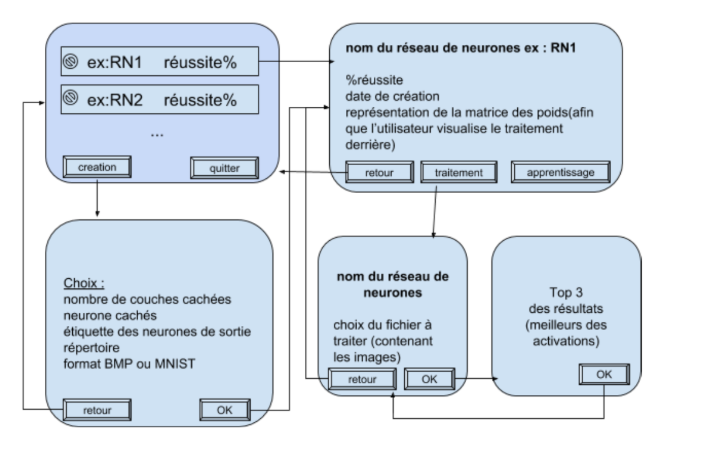
\includegraphics[height=244, width=400]{interface.png}
			\end{center}
			
\section{Explications de l'architecture :}
\subsection{Organigramme :}
			\begin{center} 
				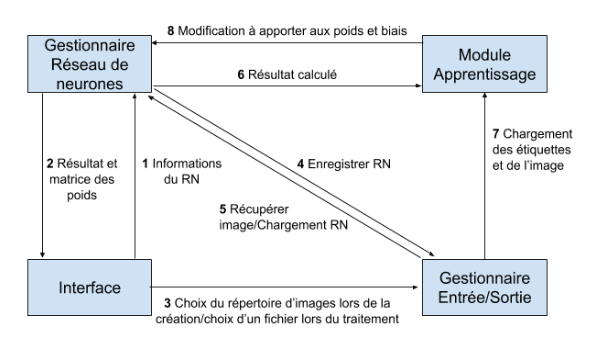
\includegraphics[height=244, width=400]{organigramme.png}
			\end{center}
	\paragraph{Connections entre les modules :}
			\begin{enumerate}
				\item Lors de la création d'un réseau de neurones, l'utilisateur choisit les différents paramètres du réseau de neurones, ces informations sont donc envoyées au gestionnaire du réseau de neurones qui va créer le réseau. Pendant la phase d'apprentissage, il faut également spécifier au réseau de neurones qu'il faut envoyer la solution calculée au module d'apprentissage.
				\item Après l'estimation d'une solution par le réseau de neurones, la solution est envoyée à l'interface. De plus, pour la visualisation de la méthode de fonctionnement du réseau, les matrices contenant les poids doivent également être envoyées à l'interface.
				\item Lors de l'apprentissage ou du traitement d'image, l'interface demande au gestionnaire d'entrée/sortie de lire un fichier à un emplacement en particulier.
				\item Après lecture d'un fichier, le contenu est envoyé au gestionnaire du réseau de neurones qui va en effectuer le traitement.
				\item Afin de sauvegarder un réseau de neurones, les différentes matrices et vecteurs contenant les poids et les biais du réseau de neurones doivent être envoyés au gestionnaire d'entrées/sorties.
				\item Lors de l'apprentissage, la solution calculée est envoyée au module d'apprentissage.
				\item Afin de permettre l'apprentissage du réseau de neurones, la solution attendue doit être récupérée puis envoyée au module d'apprentissage.
				\item Après avoir calculé les modifications à apporter aux poids et biais du réseau de neurones, celles-ci doivent être envoyé au gestionnaire du réseau de neurones afin que celui-ci les applique.
			\end{enumerate}

\section{Choix du langage :}
La programmation de notre projet a été réalisée avec le langage C. Celui-ci correspond au langage le plus adapté pour la réalisation. En effet, la nature même du langage est procédurale : il n'y a pas d'interdépendance des différents éléments de notre programme, il y a un seul algorithme complexe à développer ; il y a l'utilisation des structures de données bien spécifiques (tableaux, matrices), mais aussi la conception de notre application est plutôt linéaire. 
Ce langage C nous a apporté plusieurs avantages tout au long de la programmation :
Simplicité du langage : simple à utiliser (assimiler l'ensemble de ses mécanismes)
La puissance : langage universel, convenant aussi bien  à la programmation système qu'au codage d'algorithmes et à la représentation de structure de données complexes, au développement d'interface ou au calcul numérique.
La portabilité : portable facilement sur des systèmes différents.
La souplesse : n'impose pas de cycle particulier
L'efficacité : grâce aux variétés de ses expressions ; il permet d'optimiser à la main les sources de programmes.

\section{Description du fonctionnement global de l'application :}
L'utilisateur crée un nouveau réseau de neurone dont il veut préciser les informations (nom , nombre couches cachées, nombre de neurones par couches, choix du répertoire d'images à analyser,ainsi que la hauteur et la largeur de ces images).
L'utilisateur crée ou choisit un réseau de neurone, il a ensuite la possibilité entre l'apprentissage et le traitement.
L'apprentissage va permettre d'entraîner le réseau de neurones ce qui permettra d'effectuer un traitement d'information.
Le traitement demandera une image à reconnaître, et après exécution, envoyer les trois meilleurs résultats, c'est à dire les trois neurones de sorties avec la plus haute activation (correspondant aux étiquettes avec le plus de point communs avec l'image choisie). 

\section{Description des points délicats de la programmation :}
Propagation :
L'algorithme de propagation consiste a propager les activations de la couche d'entrée jusqu'à la couche de sortie en suivant la formule A(L) = sigmoïde( W(L) * A(L-1) + B(L) ) avec A(L) le vecteur des activations de la couche L, W(L) la matrice des poids des liaisons entre les neurones de la couche L-1 et ceux de la couche L et B(L) le vecteur des biais des neurones de la couche L.
Propagation inverse :
L'algorithme de propagation inverse va suivre un ensemble de formules afin d'ajuster les poids et les biais d'un réseau de neurones dans le but de minimiser l'erreur entre le résultat souhaité et le résultat obtenu par le réseau. Les étapes de la propagation inverse sont les suivantes :
		\begin{enumerate}
			\item Entrer un vecteur des activations correspondant à une image dans la première couche du réseau de neurones
			\item Effectuer la propagation sur le réseaux
			\item Calculer le vecteur d'erreur $δx,L=∇aCx⊙σ′(zx,L)$
			\item Pour chaque couche L calculer : $δx,l=((wl+1)Tδx,l+1)⊙σ′(zx,l)$
			\item Changer les poids et les biais de chaque couches en suivant les règles : $wl→wl−η∑xδx,l(ax,l−1)T et bl→bl−η∑xδx,l$
		\end{enumerate}
Lecture MNIST :
Afin de lire les fichiers de la base de donnée MNIST, qui sont au format IDX, nous devons d'abord récupérer : l'entête du fichier composé d'un numéro magique permettant certaines vérifications de base sur le contenu du fichier, le nombre d'image contenues dans le fichier ( lors de la lecture d'un fichier, c'est la dernière image que nous lisons, le nombre d'image est ensuite réduit de 1 puis réécrit) ainsi que la largeur et la hauteur des images. Vient ensuite le contenu des images, un octet par pixel (les images sont en noir et blanc).
Lecture BMP :
Les fichiers bmp suivent le même principe, une entête contenant diverses informations précède l'image qui utilise 3 octets pour chaque pixel pour chaque composants "`couleur"'. Contrairement au fichier idx, une seule image est présente par fichier bmp.

\section{Tableau des coûts et estimation :}
{\setlength{\tabcolsep}{0.07cm}
		\begin{center}
		\small
		\begin{tabular}{|c|c|c|c|c|}
		\hline
		Module de notre projet & Gestionnaire du Réseau de Neurones & Apprentissage & Gestionnaire d'entrées sorties & Interface\\
		\hline
		Coût prévu initialement & 155 & 150 & 75 & 310\\
		\hline
		Coût réel & 260 & 170 & 556 & 530\\
		\hline
		\end{tabular}
		\end{center}
 }
L'estimation du coût a été un travail complexe. En effet, nous avons grandement sous-estimé le coût nécessaire à la création des modules de notre application. 
De plus, la gestion des problèmes lors de la programmation a augmenté le coût de nos modules, déjà évalué lors de l'estimation. C'est ainsi que nous possédons un coût réel avec  un contraste important par rapport au coût initialement prévu.

\section{Conclusion technique et perspective :}
\subsection{Axes d'amélioration :}
	\begin{enumerate}
			\item Répartition des valeurs :
			Lors de la création d'un réseau de neurones, des valeurs sont attribuées aux poids et aux biais du réseaux. La distribution de ces valeurs ne doivent cependant pas être totalement aléatoire, en effet plus les poids et les biais sont éloignés de la valeur qui permettrait de minimiser l'erreur du réseau, plus le processus d'apprentissage, déjà très long a la base, est rallongé. 
De plus, le nombre d'exemple nécessaire augmente lui aussi, ce qui peut poser problème dans le cas ou la base de données à disposition est restreinte. 
Dans notre application, ces valeurs sont choisies aléatoirement entre -1 et 1 avec une précision maximale de 10 -2 . La manière optimale serait d'opter pour une répartition Gaussienne centré sur 0 avec une variance de 1.
			\item Taux d'apprentissage :
			Si on considère le cas d'un réseau de neurones à deux neurones, possédant donc deux paramètres
$W_1$ et $B_1$ (appelé $v_1$ et $v_2$ sur le graphe ci-dessous). On peut représenter la fonction coût en fonction de ces
deux paramètres. Cette fonction a été représentée à droite. On remarquera le point vert ainsi que la flèche verte représentant les paramètres actuelles et l'inverse du gradient de la fonction C.
Lors de l'apprentissage du réseau, l'objectif est de faire varier les paramètres en suivant l'inverse du gradient de C afin de minimiser le coût.
Cependant un autre paramètre entre en jeux : le taux d'apprentissage. Avant d'appliquer l'inverse du gradient aux paramètres , celui-ci est multiplié par le taux  d'apprentissage. 
Pour faire fonctionner la descente de gradient correctement, nous devons choisir un taux d'apprentissage suffisamment petit afin que ΔC ne soit pas positif mais suffisamment petit afin de ne pas ralentir le processus d'apprentissage.
				\begin{center} 
					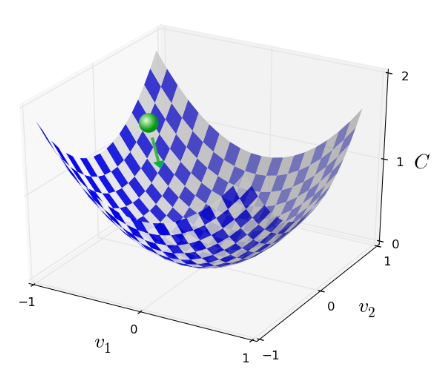
\includegraphics[height=244, width=400]{courbe.png}
				\end{center}
			\item Descente de gradient stochastique :
			Afin d'améliorer les performances de l'application, il serait possible d'opter pour la version stochastique de la descente de gradient où la rétro-propagation est effectuée sur la moyenne de l'erreur de plusieurs images et non plus sur l'erreur de chaque image.
	\end{enumerate}

\subsection{Problèmes rencontrés :}
	\begin{enumerate}
			\item Transposition de matrice :
			Transposer une matrice représentée sous la forme d'un tableau nécessiterait en c de réallouer entièrement un tableau à deux dimensions. Cette opération étant coûteuse et effectuée deux fois pour chaque couche du réseau de neurones pour chaque exemples d'apprentissage. Sachant que chaque matrices nécessitant une transposition est ensuite multipliée par une autre matrice, nous avons directement effectué la multiplication matricielle sans effectuer la transposition tout en changeant la façon de lire la matrice qui aurait dû être transposée lors de la multiplication matricielle.
			\item Lecture et Écriture d'entier dans un fichier ouvert en binaire : 
			Pour une raison qui nous est inconnue, les fonctions de lecture et d'écriture inversent tous les octets des éléments à lire ou à écrire. Ceci ne pose aucun problèmes dans le cas de caractères, cependant si on utilise un autre type,  un problème se pose. Par exemple, si un fichier comprend l'entier $1$ ($00000000000000000000000000000001$), la lecture renverra $16777216$ ($000000001000000000000000000000000$). Dans le cas de l'écriture puis de la lecture (enregistrement puis chargement d'un réseau de neurones), les octets sont inversés à l'écriture puis ré-inversé à la lecture (revenant donc à leur place initiale).
Cependant les fichier de la base de données MNIST est déjà écrite et ses octets ne sont pas inversés, il faut donc inverser à la main les octets de chaque éléments lus dans ces fichiers.
			\item Test difficiles à réaliser :
			Le test de fonctionnement de l'apprentissage est assez compliqué à réaliser car on ne connaît pas quel résultat est censé obtenir le programme. Il a donc fallu réaliser tous les calculs à la main sur un petit réseau de neurones et le test se résume donc à afficher les valeurs obtenues par le programme et à les comparer avec les résultats calculés.
			\item Interface :
			 La mise en place du module a été complexe. Il a fallu apprendre l'utilisation de la bibliothèque $GTK+2$ et suivre des tutoriels pour pouvoir par la suite l'adapter selon nos besoins.  L'utilisation des champs de saisies  pour la récupération des informations n'était pas évidente et nécessitait l'utilisation de fonctions plus avancées comme l'imbrication de VBox entre elles ainsi que l'utilisation de plusieurs listes pour les récupérations . 
Il y a aussi un problèmes de fenêtres superposées,  pour le résoudre nous avons créés des fonctions de destructions qui testaient à chaque fois la liste des fenêtres, détruisait l'ancienne élément et passait au suivant.
Nous avons déclaré une structure INFO\_FENETRE pour les variables communes aux fenêtres comme window, ainsi que d'autres pour stocker et récupérer toutes les informations circulant dans les fenêtres pour pouvoir les utiliser par la suite.      
	\end{enumerate}

\section{Conclusion organisation interne :}
Pour ce qui est de l'organisation interne, nous avons appris à gérer un projet et à faire face au difficulté ensemble. C'est la bonne cohésion et une organisation plutôt bonne au sein du groupe  qui nous a permis de mener notre projet à terme. 
Nous avons saisis qu'il était essentiel d'évaluer les connaissances de chacun. Ainsi, nous avons beaucoup travaillé durant les séances et en dehors.  De plus, nous avons appris qu'un point important est la communication lorsqu'on travaille en groupe,. En effet, même si étant pratique, une discussion par messagerie instantanée ne peut se substituer à une réunion en face à face pour nous permettre de faire le points sur nos tâches régulièrement. 

\section{Conclusion du rapport :}
Pour conclure, c'est la première fois que nous travaillons en groupe en étant aussi nombreux sur un projet de cette ampleur avec un but bien défini. De notre point de vue, nous avons consolidé nos connaissances générales et appris à réaliser un programme de manière correct. 
Notre code est conforme à sa spécification et efficace, ce qui nous a permis de rendre notre programme maintenable et réutilisable. 
Nous sommes dans l'ensemble satisfait de la réalisation effectuée. Nous avons réussi à exploiter au mieux notre temps, en partageant les tâches et en se concertant sur toutes les décisions importantes, afin de pouvoir finaliser nos objectifs dans les temps.

\end{document}
